\documentclass{templateNote}

\usepackage{enumitem}
\usepackage{overpic}
\usepackage{soul}

\newcommand{\newparagraph}{\par\vspace{\baselineskip}\noindent}

\newcommand{\hlcolor}[2]{{\sethlcolor{#1}\hl{#2}}}
\definecolor{Verde}{RGB}{170,239,31}
\definecolor{Morado}{RGB}{127,0,255}
\definecolor{Celeste}{RGB}{0,191,255}
\definecolor{Salmon}{RGB}{255,0,157}

\begin{document}

\imagenlogoU{img/LogoElNube.png}
\linklogoU{https://github.com/MarceloPazPezo}
\imagenlogoD{img/LogoNGM.png}
\linklogoD{https://github.com/NicoGomezM}
\linkQRDoc{https://github.com/MarceloPazPezo/MyRepo/blob/main/Icinf/Semestre\%207/Gesti\%C3\%B3n\%20Estrat\%C3\%A9gica/Certamen\%201/Certamen-1.pdf}
\titulo{Certamen 1}
\asignatura{Gestión Estratégica}
\autor{
Nicol\'as G\'omez\\
Marcelo Paz
}
\vDoc{1.0.1}

% Metadatos del PDF
\title{[\asignatura]-\titulo}
\author{
    \autor
}
\portada
\margenes % Crear márgenes

\section{Introducci\'on a la G.E.}
\subsection{Conceptos B\'asicos}
\begin{itemize}
    \item Estado $\neq$ Gobierno.
    
    \item \textbf{Estado:} Conjunto de personas que habitan un pa\'is.
    
    \item \textbf{Gobierno:} Administraci\'on del Estado.
    
    \item \textbf{Congreso:} Poder Legislativo(El que hace las leyes).
    
    \item \textbf{Estado de Derecho:} Las decisiones son tomadas por el congreso.
    
    \item \textbf{Estrategia:} Es un plan de acci\'on que se dise\~na para alcanzar un objetivo.
    
    \item \textbf{Gesti\'on:} Es el proceso de planificar, organizar, dirigir y controlar los recursos de una organizaci\'on.
    
    \item \textbf{Gesti\'on Estrat\'egica:} Es el proceso de formulaci\'on e implementaci\'on de estrategias.
    
    \item \textbf{Stakeholders:} \hl{Personas que tienen inter\'es en la organizaci\'on.}
    
    \item \textbf{Misi\'on:} Prop\'osito gen\'erico acorde con las necesidades/expectativas de los stakeholders. (Raz\'on de ser)
    
    \item \textbf{Visi\'on:} Imagen futura de la organizaci\'on. (A donde queremos llegar)
    
    \item \textbf{Meta:} Afirmaci\'on gen\'erica del prop\'osito.
    
    \item \textbf{Objetivo:} Cuanti ficaci\'on de la meta.
    
    \item \textbf{N\'ucleo de competencias:} Recursos, procesos o habilidades que proporcionan ventaja competitiva.
    
    \item \textbf{Estrategias (Def. PPT):} Direcci\'on a largo plazo.
    
    \item \textbf{Arquitectura estrat\'egica:} Combinaci\'on de recursos, procesos y competencias para aplicar la estrategia.
    
    \item \textbf{Control:} Control de las acciones para lograr efectividad de las estrategias y acciones o si es necesario, modificar estrategias y/o acciones.
\end{itemize}

\newpage
\subsection{Importancia de la G.E.}
En palabras simples, la G.E. es importante para la supervivencia de una organizaci\'on, pues nos permite anticipar y adaptarnos a los cambios del entorno, adem\'as de aprovechar las oportunidades y minimizar las amenazas.

\section{Tipos de Organizaciones}
\subsection{Seg\'un su tama\~no o Magnitud}
\begin{itemize}
    \item \textbf{Microempresa:} 1 a 9 trabajadores.
    
    \item \textbf{Peque\~na empresa:} 10 a 49 trabajadores.
    
    \item \textbf{Mediana empresa:} 50 a 199 trabajadores.
    
    \item \textbf{Gran empresa:} 200 o m\'as trabajadores.
\end{itemize}

\subsection{Seg\'un su actividad o giro}
\begin{itemize}
    \item \textbf{Primarias:} Agricultura, ganader\'ia, pesca, miner\'ia.
    
    \item \textbf{Secundarias:} Industria, construcci\'on.
    
    \item \textbf{Terciarias:} Comercio, servicios.
\end{itemize}

\subsection{Seg\'un el sector econ\'omico al que pertenece}
\begin{itemize}
    \item \textbf{Microempresa:} Hasta 1000 UF.
    
    \item \textbf{Peque\~na empresa:} Hasta 25.000 UF.
    
    \item \textbf{Mediana empresa:} Hasta 100.000 UF.
    
    \item \textbf{Gran empresa:} M\'as de 100.000 UF.
\end{itemize}

\subsection{Seg\'un al origen de su capital}
\begin{itemize}
    \item \textbf{P\'ublicas:} Capital del Estado.
    
    \item \textbf{Privadas:} Capital de particulares.
    
    \item \textbf{Mixtas:} Capital del Estado y de particulares.
\end{itemize}

\subsection{Seg\'un su constituci\'on jur\'idica}
\begin{itemize}
    \item \textbf{Empresario individual (autónomo):} Una sola persona posee la empresa y es responsable ilimitadamente de las deudas.
    
    \item \textbf{Sociedad colectiva:} Dos o más socios comparten la gestión y responden \newline ilimitadamente de las deudas.
    
    \item \textbf{Sociedad comanditaria:} Combina socios colectivos que gestionan y responden ilimitadamente y socios comanditarios que solo aportan capital y su responsabilidad se limita a su aportación.
    
    \item \textbf{Sociedad de responsabilidad limitada (SRL o SL):} La responsabilidad está limitada al capital aportado por los socios.
    
    \item \textbf{Sociedad anónima (SA):} El capital está dividido en acciones, y la responsabilidad de los accionistas se limita al valor de sus acciones.
    
    \item \textbf{Sociedad por acciones simplificada (SAS):} Es una variante moderna que permite una gran flexibilidad en su constitución y gestión.
\end{itemize}

\subsection{Seg\'un su \'ambito de la actividad}
\begin{itemize}
    \item \textbf{Local:} Desarrollan su actividad en una localidad.
    
    \item \textbf{Regional:} Desarrollan su actividad en una regi\'on.
    
    \item \textbf{Nacional:} Desarrollan su actividad en todo el pa\'is.
    
    \item \textbf{Multinacional:} Desarrollan su actividad en varios pa\'ises.
    
    \item \textbf{Global:} Desarrollan su actividad en todo el mundo.
\end{itemize}

\subsection{Seg\'un el destino de las ganancias}
\begin{itemize}
    \item \textbf{Con fines de lucro:} Objetivo de obtener ganancias.
    
    \item \textbf{Sin fines de lucro:} Objetivo de satisfacer necesidades de la comunidad.
    \begin{itemize}
        \item Fundaciones.
        
        \item Corporaciones.
    \end{itemize}
\end{itemize}

\newpage
\section{Administraci\'on Estrat\'egica}
\subsection{Definici\'on}
La estrategia de negocios como direcci\'on y alcance de una organizaci\'on a largo plazo, permite \hlcolor{orange!50}{obtener ventajas competitivas} en un entorno cambiante, mediante una configuraci\'on de recursos que permite hacer frente a los mercados y satisfacer las necesidades de los \textbf{stakeholders}.

\subsection{Procesos de la A.E.}\label{sec:ref1}
\begin{itemize}
    \item \hlcolor{orange!50}{\textbf{Selecci\'on de la misi\'on y objetivos.}}
    
    \item \hlcolor{orange!50}{\textbf{An\'alisis del entorno competitivo externo (Oportunidades y Amenazas).}}
    
    \item \hlcolor{orange!50}{\textbf{An\'alisis de los recursos internos (Fortalezas y Debilidades).}}
    
    \item \hlcolor{orange!50}{\textbf{Formulaci\'on de estrategias (Decidir el camino de la empresa).}}
    
    \item \hlcolor{orange!50}{\textbf{Implementaci\'on de estrategias (Como y quien hace las cosas).}}
    
    \item \hlcolor{orange!50}{\textbf{Evaluaci\'on y control (Cheque antes, durante y despu\'es del proceso).}}
\end{itemize}

\subsection{Tri\'angulo de la A.E.}
\vspace{2cm}
\begin{center}
    \begin{overpic}[width=0.9\textwidth]{img/triangulo.png}
        \put(41,40){\hyperref[sec:analisisEstrategico]{\phantomsection\hspace{6.3em}\raisebox{0pt}[0.4cm][0.63cm]{}}}
        \put(17,16){\hyperref[sec:eleccionEstrategica]{\phantomsection\hspace{6.3em}\raisebox{0pt}[0.4cm][0.63cm]{}}}
        \put(24,54){\hyperref[subsec:entorno]{\phantomsection\hspace{4.8em}\raisebox{0pt}[0.4cm][0.48cm]{}}}
        % \put(17,16){\hyperref[sec:eleccionEstrategica]{\phantomsection\colorbox{yellow}{\hspace{5.7em}\raisebox{0pt}[0.4cm][0.63cm]{}}}}
    \end{overpic}
\end{center}

\newpage
\section{Análisis estratégico}\label{sec:analisisEstrategico}
\begin{itemize}
    \item \textbf{El entorno:} Conjunto de factores que rodean a la empresa y que influyen en su funcionamiento.
    
    \item \textbf{Expectativas y propósitos:} Objetivos que se desean alcanzar.
    
    \item \textbf{Recursos:} Elementos que se utilizan para alcanzar los objetivos.
    
    \item \textbf{Competencias:} Habilidades y destrezas que permiten alcanzar los objetivos.
    
    \item \textbf{Capacidades:} Conjunto de recursos y competencias que permiten alcanzar los objetivos.
\end{itemize}

\subsection{Entorno}\label{subsec:entorno}
\noindent Tanto \hlcolor{Celeste!30!white}{el entorno empresarial como el económico global se ven afectados por distintos factores frente a los cuales estos entes deben enfrentarse a la \textbf{necesidad de una reconsideración} de sus estrategias.} Algunos de estos factores son:

\begin{itemize}
    \item \hlcolor{Celeste!30!white}{Liberalización:} Reducción de restricciones comerciales de parte del gobierno lo cual facilita el libre comercio y la inversion.
    
    \item \hlcolor{Celeste!30!white}{Cambios estructurales:} Cambios duraderos y significativos en la estructura de la economía, como la globalización.
    
    \item \hlcolor{Celeste!30!white}{Competencia global:} Competencia entre empresas de distintos países.
    
    \item \hlcolor{Celeste!30!white}{Bloques de comercio:} Agrupaciones de países que establecen acuerdos comerciales.
    
    \item \hlcolor{Celeste!30!white}{Discontinuidad tecnológica:} Cambios tecnológicos que afectan la forma de hacer negocios.
    
    \item \hlcolor{Celeste!30!white}{Exceso de capacidad:} Producción de bienes o servicios en exceso.
    
    \item \hlcolor{Celeste!30!white}{Fusiones y adquisiciones:} Compra de una empresa por otra.
    
    \item \hlcolor{Celeste!30!white}{Preocupación medioambiental:} Preocupación por el impacto ambiental de las empresas.
    
    \item \hlcolor{Celeste!30!white}{Expectativas cambiantes de los clientes:} Cambios en las preferencias de los consumidores.
    
    \item \hlcolor{Celeste!30!white}{Menor proteccionismo:} Menos políticas proteccionistas por parte de los gobiernos, lo que promueve un mercado más abierto y competitivo.
\end{itemize}

\subsubsection{Exploración ambiental de la organizacion}
\noindent La exploración ambiental de la organización \hlcolor{Verde}{es un proceso que permite identificar y analizar los factores del entorno que pueden afectar a la empresa.}
Este proceso se lleva a cabo a través de la \hlcolor{Verde}{recolección de información y el análisis de los datos obtenidos.} Algunos de los ambientes \textbf{críticos} existentes son:
\begin{itemize}
    \item \hlcolor{Verde}{\textbf{Ambiente de clientes:}} Comprender y analizar las características y comportamientos de los clientes actuales y potenciales, incluyendo variables demográficas, y mantener comunicación e intercambio de información para ganar su confianza y establecer relaciones comerciales.
    
    \item \hlcolor{Verde}{\textbf{Ambiente competidores:}} Analizar la identidad, motivos, fortalezas, debilidades y conductas de las empresas competidoras, así como sus métodos para llegar a los clientes deseados. Incluso sus clientes pueden volverse competidores (Modelo de Rivalidad Ampliada).
    
    \item \hlcolor{Verde}{\textbf{Cambio de proveedores:}} Los cambios de proveedores impactan los costos de inversión, precios, demanda, márgenes de contribución, suministros, procesos de producción, requisitos de inversión, costos y disponibilidad.
    
    \item \hlcolor{Verde}{\textbf{Ambiente competitivo:}} El ambiente competitivo influye en la adopción de nuevas tecnologías, afectando costos y calidad de productos; la entrada de nuevos competidores impacta precios, participación de mercado y márgenes de contribución; y el lanzamiento de nuevos productos modifica la demanda y los gastos en publicidad.
    
    \item \hlcolor{Verde}{\textbf{Cambios en el mercado:}} Los cambios en el mercado incluyen nuevos usos de productos que afectan la demanda y utilización de capacidades, nuevos mercados que influyen en los canales de distribución, demanda y uso de capacidades, y la obsolescencia de productos que impacta precios, demanda y utilización de capacidades.
    
    \item \hlcolor{Verde}{\textbf{Ambiente económico:}} El ambiente económico se ve afectado por las tasas de interés, las tasas de cambio y los cambios en el ingreso per cápita, los cuales influyen en la expansión económica, la demanda interna y externa, así como en los beneficios empresariales.
    
    \item \hlcolor{Verde}{\textbf{Ambiente tecnológico:}} El ambiente tecnológico influye en los costos y la calidad de los productos, la aparición de nuevos competidores, la determinación de precios, el desarrollo de nuevos productos, los cambios en los canales de distribución, la demanda y la utilización de capacidades, así como en la obsolescencia de productos.
    
    \item \hlcolor{Verde}{\textbf{Ambiente social:}} Los cambios en las preferencias de los clientes y las tendencias demográficas afectan la demanda y el diseño de productos, mientras que la incorporación al mercado laboral influye en los costos. La profesionalización del personal incide en los costos y la productividad, y la globalización impacta en los costos, la demanda y la competitividad.
    
    \item \hlcolor{Verde}{\textbf{Ambiente politico:}} Los cambios en la legislación y regulación afectan los costos, la demanda y la competitividad, mientras que la estabilidad política influye en la inversión y la demanda.
    
    \item \hlcolor{Verde}{\textbf{Ambiente legal:}} Los cambios en la legislación y regulación afectan los costos, la demanda y la competitividad, mientras que la estabilidad política influye en la inversión y la demanda.
    
    \item \hlcolor{Verde}{\textbf{Ambiente físico:}} Los cambios en el ambiente físico afectan la demanda y la utilización de capacidades, mientras que la disponibilidad de recursos naturales influye en los costos y la competitividad.
\end{itemize}

\subsection{Estrategia competitiva}
\noindent Búsqueda de posición favorable en uno o mas sectores del mercado; Las ventajas competitivas de una empresa se basan principalmente en la capacidad de la empresa para ofrecer un valor único y significativo a sus clientes. Inciden en la elección de la estrategia competitiva:
\begin{itemize}
    \item \textbf{Atractivo del sector} para obtener utilidades a largo plazo y los factores determinantes.
    
    \item Determinantes de una \textbf{posición competitiva} relativa dentro de un sector especifico.
    
    \item Ambos factores anteriores son dinámicos y cambian con el tiempo.
\end{itemize}

\subsection{Modelos estratégicos basados en el sector industrial}

\subsubsection{Modelo competitivo (Atractivo del sector)}
\noindent Se basa en las fuerzas que mueven a la competencia en un sector industrial, las cuales determinan la rentabilidad a largo plazo de las empresas en dicho sector.

\newparagraph
\noindent\underline{\textbf{Fuerzas que mueven a la competencia}}
\begin{itemize}[label=$-$]
    \item La rivalidad ampliada determina el grado de la competencia dentro de la industria.
    \item El éxito de una empresa en un sector industrial dependerá de su propia estrategia.
    \item El estudio del modelo Porter permite:
    \begin{itemize}
        \item Definir una estrategia competitiva mas ad-hoc.
        \item Buscar una posición del sector donde la empresa pueda defenderse de las 5 fuerzas o usarlas a su favor.
    \end{itemize} 
\end{itemize}
\textbf{Las 5 fuerzas de Porter}
\begin{center}
    \begin{overpic}[width=0.9\textwidth]{img/FuerzasPorter.png}
        \put(30,62){\hyperlink{competidoresPotenciales}{\phantomsection\hspace{4.5em}\raisebox{0pt}[0.4cm][0.35cm]{}}}
        \put(30,9.5){\hyperlink{sustitutos}{\phantomsection\hspace{4.5em}\raisebox{0pt}[0.4cm][0.35cm]{}}}
        \put(26,43.7){\hyperlink{rivalidad}{\phantomsection\hspace{7.4em}\raisebox{0pt}[0.4cm][2.65cm]{}}}
        \put(60,35.5){\hyperlink{clientes}{\phantomsection\hspace{4.5em}\raisebox{0pt}[0.4cm][0.35cm]{}}}
        \put(0.5,35.5){\hyperlink{proveedores}{\phantomsection\hspace{4.5em}\raisebox{0pt}[0.4cm][0.35cm]{}}}
        % \put(17,16){\hyperref[sec:eleccionEstrategica]{\phantomsection\colorbox{yellow}{\hspace{5.7em}\raisebox{0pt}[0.4cm][0.63cm]{}}}}
    \end{overpic}
\end{center}
\newpage
\begin{itemize}
    \item \hypertarget{competidoresPotenciales}{\hl{Amenaza de ingreso de nuevos competidores potenciales (ANE)}}
    \begin{itemize}
        \item Características:
        \begin{itemize}
            \item Aporta capacidad adicional.
            \item Nuevo competidor altera participación del mercado.
        \end{itemize}
        \item Consecuencias:
        \begin{itemize}
            \item Disminución de precios.
            \item Aumento de costos.
            \item Reducción rentabilidad.
        \end{itemize}
    \end{itemize}
    \item \hypertarget{sustitutos}{\hl{Amenaza de productos sustitutos (APS)}}
    \begin{itemize}
        \item Características:
        \begin{itemize}
            \item Producto sustituto reemplaza a otro.
            \item Producto sustituto reduce rentabilidad.
        \end{itemize}
        \item Consecuencias:
        \begin{itemize}
            \item Si el precio de los productos es alto, los \\clientes optaran por el producto sustituto.
        \end{itemize}
    \end{itemize}
    \item  \hypertarget{rivalidad}{\hl{Rivalidad competidores existentes (RC)}}
    \begin{itemize}
        \item Características:
        \begin{itemize}
            \item Surge presión u oportunidad para mejorar posición.
        \end{itemize}
        \item Consecuencias:
        \begin{itemize}
            \item Aumento competencia via precios.
            \item Batallas publicitarias.
        \end{itemize}
    \end{itemize}

    \item \hypertarget{clientes}{\hl{Poder negociador de los clientes (PNC)}}
    \begin{itemize}
        \item Características:
        \begin{itemize}
            \item Clientes pueden forzar reducción de precios.
            \item Exigencia por mayor calidad de productos/servicios.
        \end{itemize}
        \item Consecuencias:
        \begin{itemize}
            \item Aumento competencia entre competidores.
        \end{itemize}
    \end{itemize}
    \item \hypertarget{proveedores}{\hl{Poder negociador de los proveedores (PNP)}}
    \begin{itemize}
        \item Características:
        \begin{itemize}
            \item Proveedores pueden forzar aumento de precios.
            \item Proveedores pueden reducir calidad de productos/servicios.
            \item Asociación proveedores fuera de la industria.
        \end{itemize}
        \item Consecuencias:
        \begin{itemize}
            \item Fijación precio y calidad de insumos adquiridos por la industria.
        \end{itemize}
    \end{itemize}
\end{itemize}

\newpage
\subsubsection{Porfolio de mercado (BCG)}
\subsection{Elementos que dan valor a la estrategia}
\begin{itemize}
    \item Recursos limitados.
    \item Comportamiento competidor.
    \item Compromiso irreversible recursos.
    \item Necesidad coordinación acciones a distancia en el tiempo.
    \item Incertidumbre acerca control de iniciativa.
    \item Percepciones reciprocas entre adversarios.
\end{itemize}

\subsection{Requisitos para el desarrollo de una estrategia}
\begin{itemize}
    \item Conocimientos.
    \item Capacidad para la integración.
    \item Pericia en el análisis de sistemas para comprender racionalidad, periodicidad, posibilidades y consecuencias inmediatas/futuras.
    \item Imaginación y lógica para elegir entre alternativas.
    \item Control de recursos mas allá de la necesidad inmediata.
    \item Capacidad de renunciar a beneficios inmediatos por beneficios futuros.
\end{itemize}

\subsection{Herramientas para el desarrollo de estrategias}
\subsubsection{Análisis competitivo}
\begin{itemize}
    \item \hlcolor{Salmon!50!white}{\textbf{Análisis FODA}}
    \begin{itemize}
        \item \hlcolor{Salmon!50!white}{\textbf{Fortalezas:}} Ventajas con respecto a otras empresas las cuales mejoro o potencio.
        \item \hlcolor{Salmon!50!white}{\textbf{Oportunidades:}} Situaciones que ofrece el entorno en las cuales la empresa puede obtener algún tipo de beneficio.
        \item \hlcolor{Salmon!50!white}{\textbf{Debilidades:}} Implican costos o resultados negativos en su entorno, se buscan minimizar o eliminar.
        \item \hlcolor{Salmon!50!white}{\textbf{Amenazas:}} Situaciones presentes en el entorno que pueden afectar negativamente a la empresa, ante las cuales se prevenga o prepare.
    \end{itemize}
\end{itemize}

\newpage
\subsubsection{Análisis de cartera de actividades}
\begin{itemize}
    \item \textbf{Matrices de Planificación}
    \begin{itemize}
        \item \hlcolor{Morado!50!white}{\textbf{Matriz de crecimiento-participación:}} Analizar como funcionaria nuestra empresa en el mercado.
        \begin{itemize}
            \item Factores externos: Crecimiento del mercado.
            \item Factores internos: Participación relativa en el mercado. \\\\
            \textbf{Matriz BCG} (Boston Consulting Group)
            \begin{itemize}
                \item \hlcolor{Morado!50!white}{\textbf{Estrellas:}} Productos con alta participación en el mercado y alto crecimiento. \textbf{(Relevar a las vacas lecheras)}
                \item \hlcolor{Morado!50!white}{\textbf{Interrogantes:}} Productos con baja participación en el mercado y alto crecimiento. \textbf{(Desarrollarse o retirarse)}
                \item \hlcolor{Morado!50!white}{\textbf{Vacas lecheras:}} Productos con alta participación en el mercado y bajo crecimiento. \textbf{(Cosechar utilidades)}
                \item \hlcolor{Morado!50!white}{\textbf{Perros:}} Productos con baja participación en el mercado y bajo crecimiento. \textbf{(Retirarse o sobrevivir)}
            \end{itemize}
            \begin{figure}[H]
                \centering
                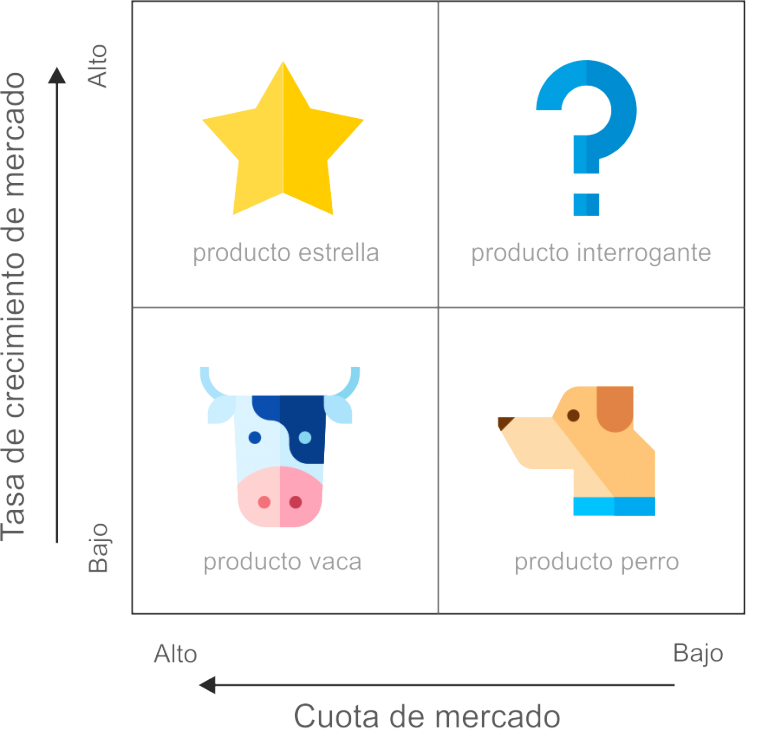
\includegraphics[width=0.7\textwidth]{img/matriz_bcg-768x803.png}
            \end{figure}
        \end{itemize}

        \newpage
        \item \textbf{Matriz atractivo de la industria-fortaleza del negocio:} Analizar la industria, ver competencia y ventaja competitiva.
        \begin{itemize}
            \item Factores externos: Atractivo de la industria.
            \item Factores internos: Fuentes de ventaja competitiva.
        \end{itemize}
        \begin{figure}[H]
            \centering
            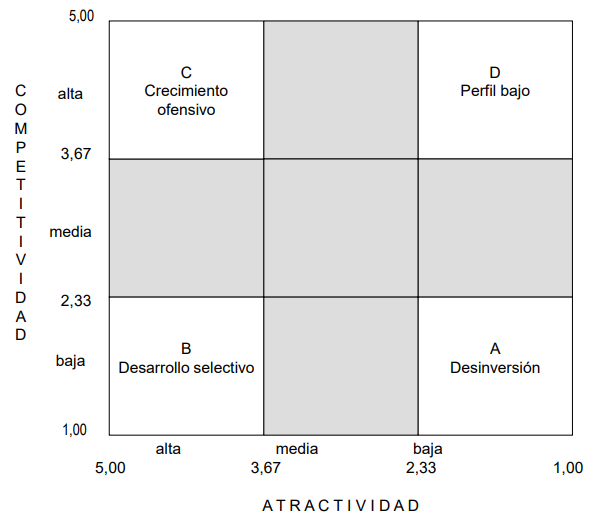
\includegraphics[width=0.7\textwidth]{img/matriz_atractivo.png}
        \end{figure}
        \item \textbf{Matriz Ciclo de vida:} Analizar el tiempo de respuesta del consumidor con respecto a un producto o servicio.
        \begin{itemize}
            \item Factores externos: Madurez de la industria.
            \item Factores internos: Medición general de la posición del negocio.
        \end{itemize}
        \item \textbf{Matriz tamaño ventaja competitiva:} Análisis especifico de nuestra ventaja con respecto a otras empresas.
        \begin{itemize}
            \item Factores externos: Formas de competir (oportunidades de diversificación).
            \item Factores internos: Tamaño/sostenibilidad de la/s ventaja/s competitiva/s.
        \end{itemize}
        \item \textbf{Matriz rentabilidad:} Comparación entre la inversion y la utilidad. 
        \begin{itemize}
            \item Factores externos: Potencial del crecimiento del mercado; Costo de capital.
            \item Factores internos: Rentabilidad; Generación de fondos.
        \end{itemize}
    \end{itemize}
\end{itemize}

\newpage
\subsubsection{Análisis de la cadena de valor}
\begin{itemize}
    \item \hlcolor{red!50!white}{\textbf{Ciclo de vida}}
    \begin{itemize}
        \item \hlcolor{red!50!white}{\textbf{Introducción:}} Producto entrando en el mercado.
        \item \hlcolor{red!50!white}{\textbf{Aceptación:}} Producto comienza a ser aceptado por el mercado objetivo.
        \item \hlcolor{red!50!white}{\textbf{Madurez:}} Producto se estabiliza en el mercado y alcanza su punto máximo de ventas.
        \item \hlcolor{red!50!white}{\textbf{Saturación:}} Producto comienza a perder ventas.
        \item \hlcolor{red!50!white}{\textbf{Obsolescencia:}} Producto deja de ser vendido o el nivel de ventas llega al mínimo (Productos Perros).
    \end{itemize}
\end{itemize}
\begin{center} 
    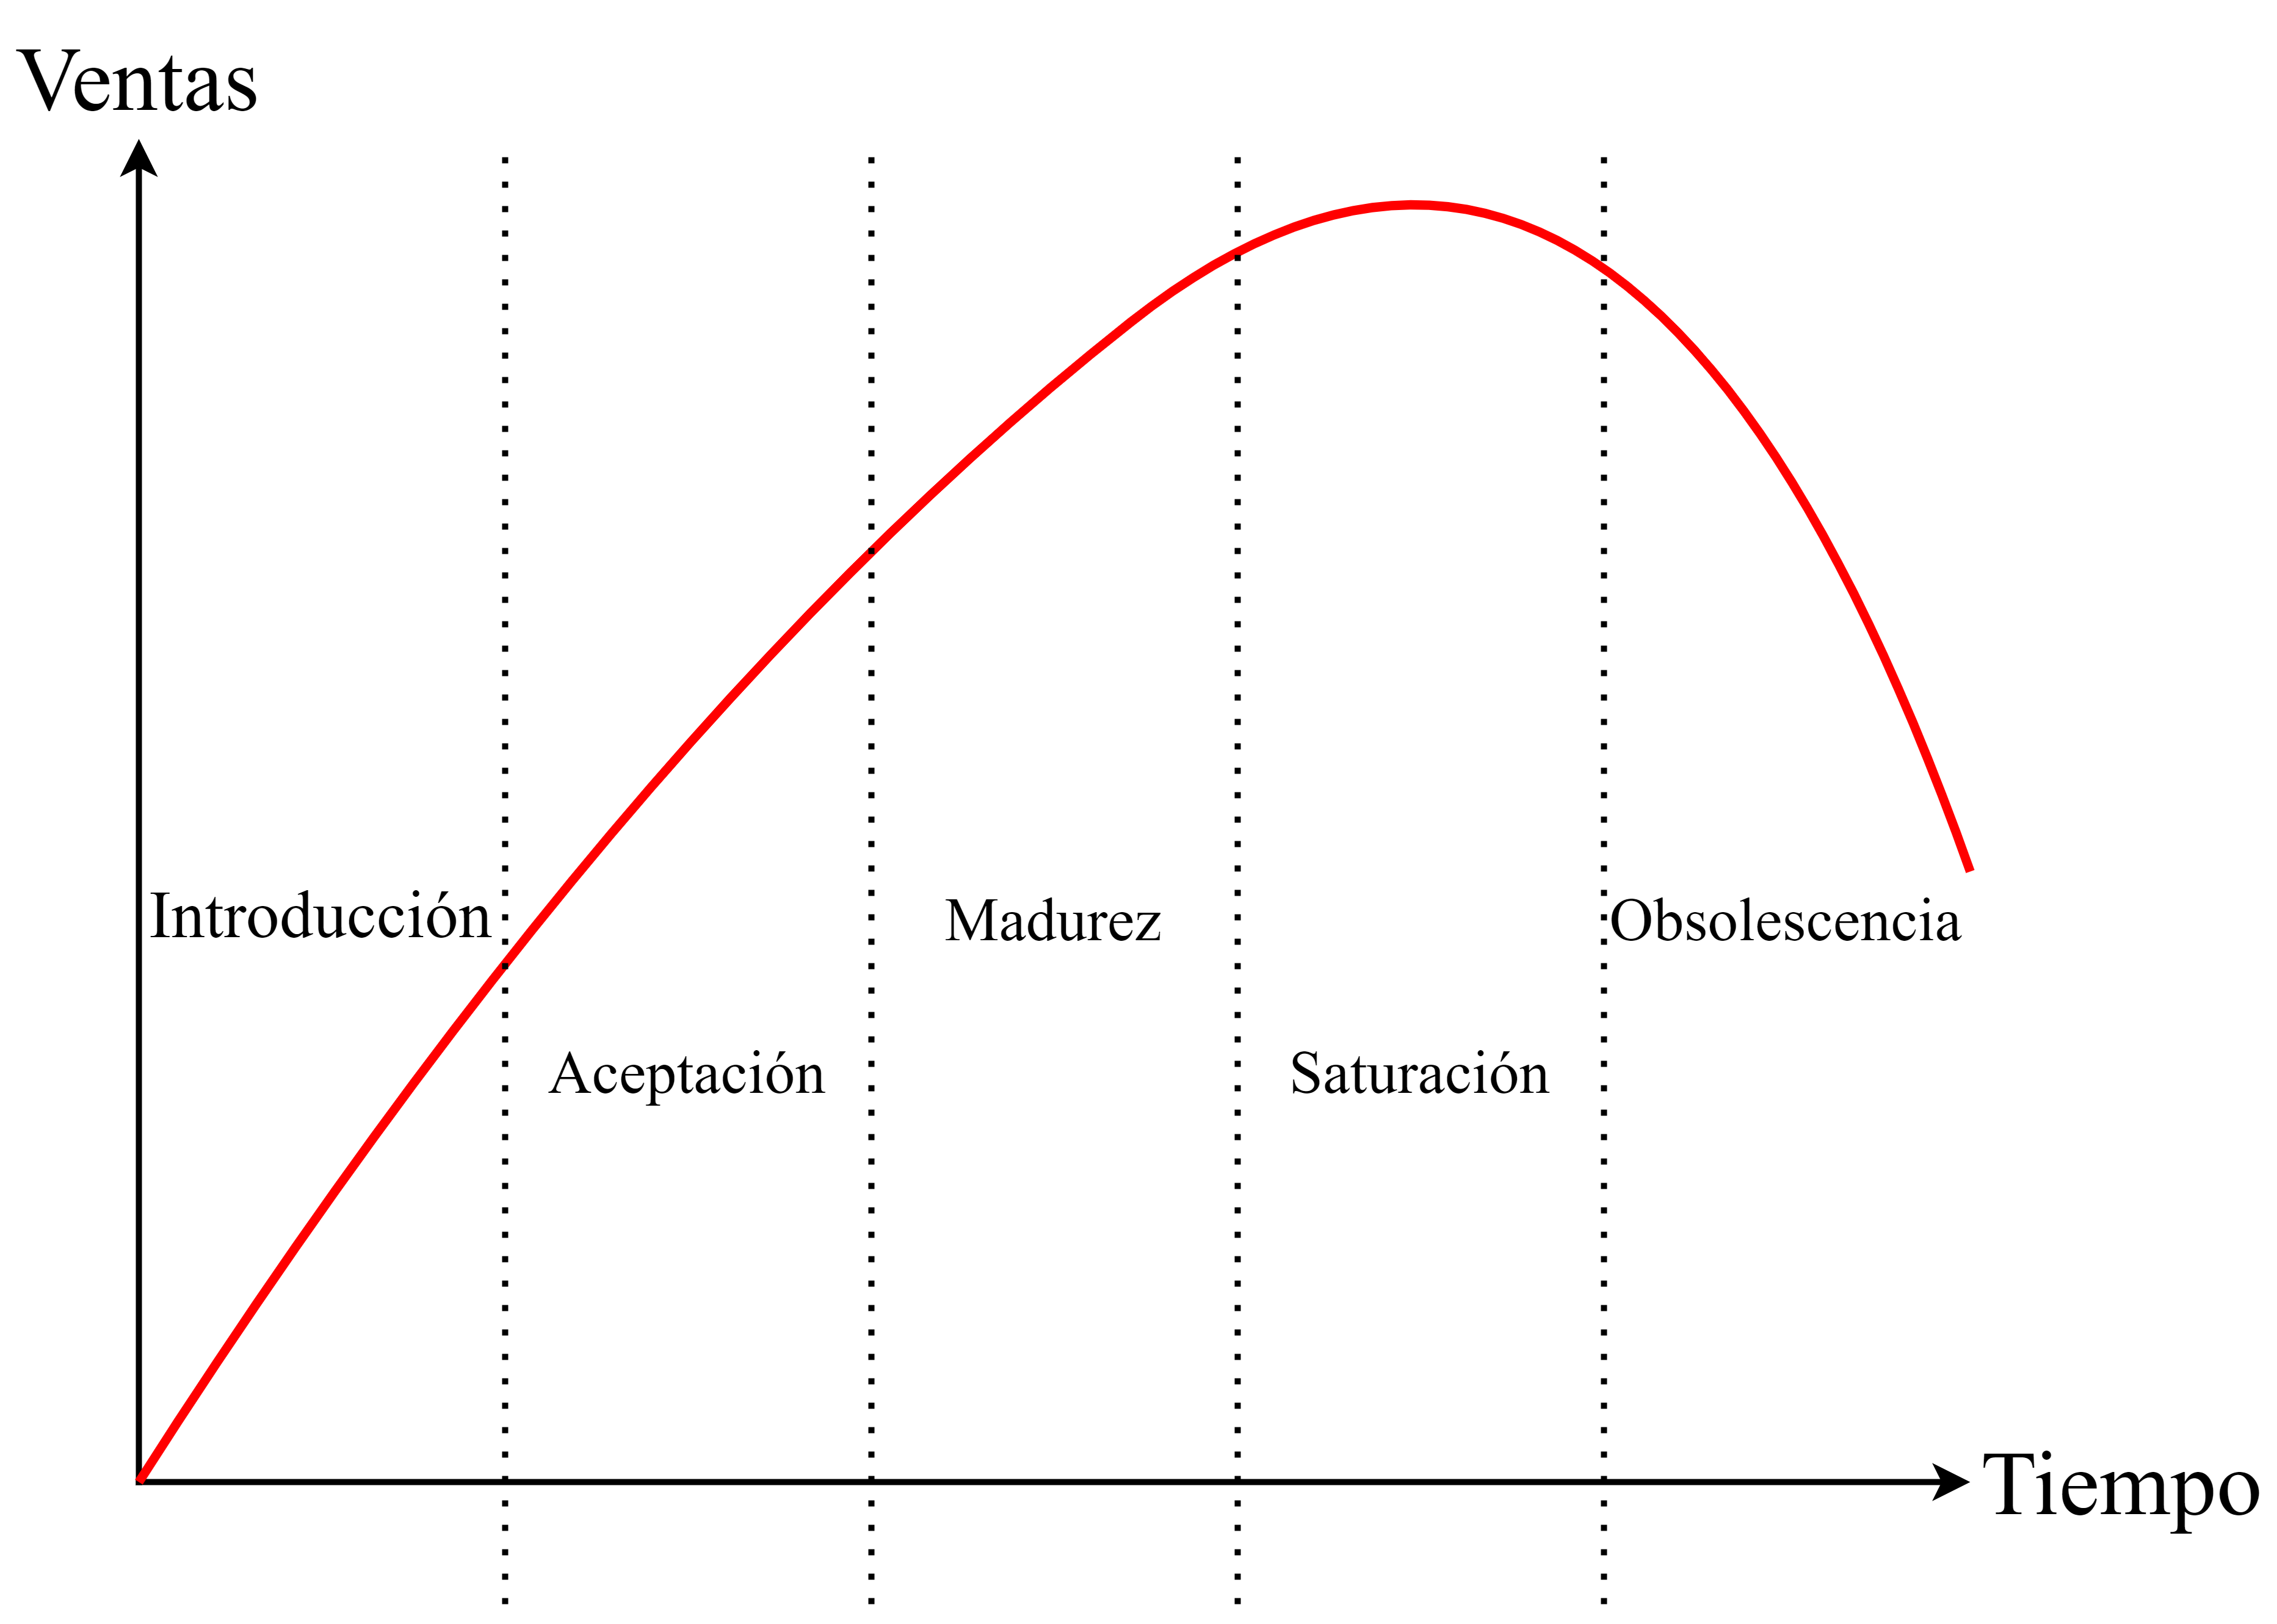
\includegraphics[width=0.8\textwidth]{img/CicloVida.png}
\end{center}
\subsubsection{Elección de estrategia}
\noindent Para elegir la estrategia a implementar, es imprescindible haber realizado previamente alguno de los análisis mencionados. Una vez completados estos análisis, las estrategias disponibles son:
\begin{itemize}
    \item Estrategia competitiva (genérica)
    \item Estrategia de crecimiento (Dinero) 
    \item Estrategia de desarrollo (Calidad de vida/productos)
\end{itemize}

\newpage
\subsection{Negocios}
\subsubsection{Categoría de negocios}
\begin{itemize}
    \item \textbf{Volumen:} Alcanzar el punto preciso del mínimo costo y liderar en ventas.
    \item \textbf{Especialización:} Centrarse en un punto del mercado y ser el mejor en ese punto o cubrir todo el mercado con productos con características únicas.
    \item \textbf{Fragmentada:} Llevar a cabo varias formas de competencias, teniendo en cuenta fuerzas relativas y competencias únicas.
    \item \textbf{Estancamiento:} Sobrevivir en el mercado a través de la reducción de costos y maximización de la productividad
\end{itemize}

\subsubsection{Lógica de negocios}
\begin{itemize}
    \item \textbf{Lógica del cliente:} Como tener acceso a los clientes.
    \item \textbf{Lógica del producto:} Oferta diferenciada que se lleva al mercado.
    \item \textbf{Lógica económica:} Obtención de beneficios o satisfacer los criterios establecidos de beneficio económico.
    \item \textbf{Lógica estructural:} Organización necesaria para que las 3 lógicas anteriores operen en conjunto.
\end{itemize}

\begin{figure}[H]
    \centering
    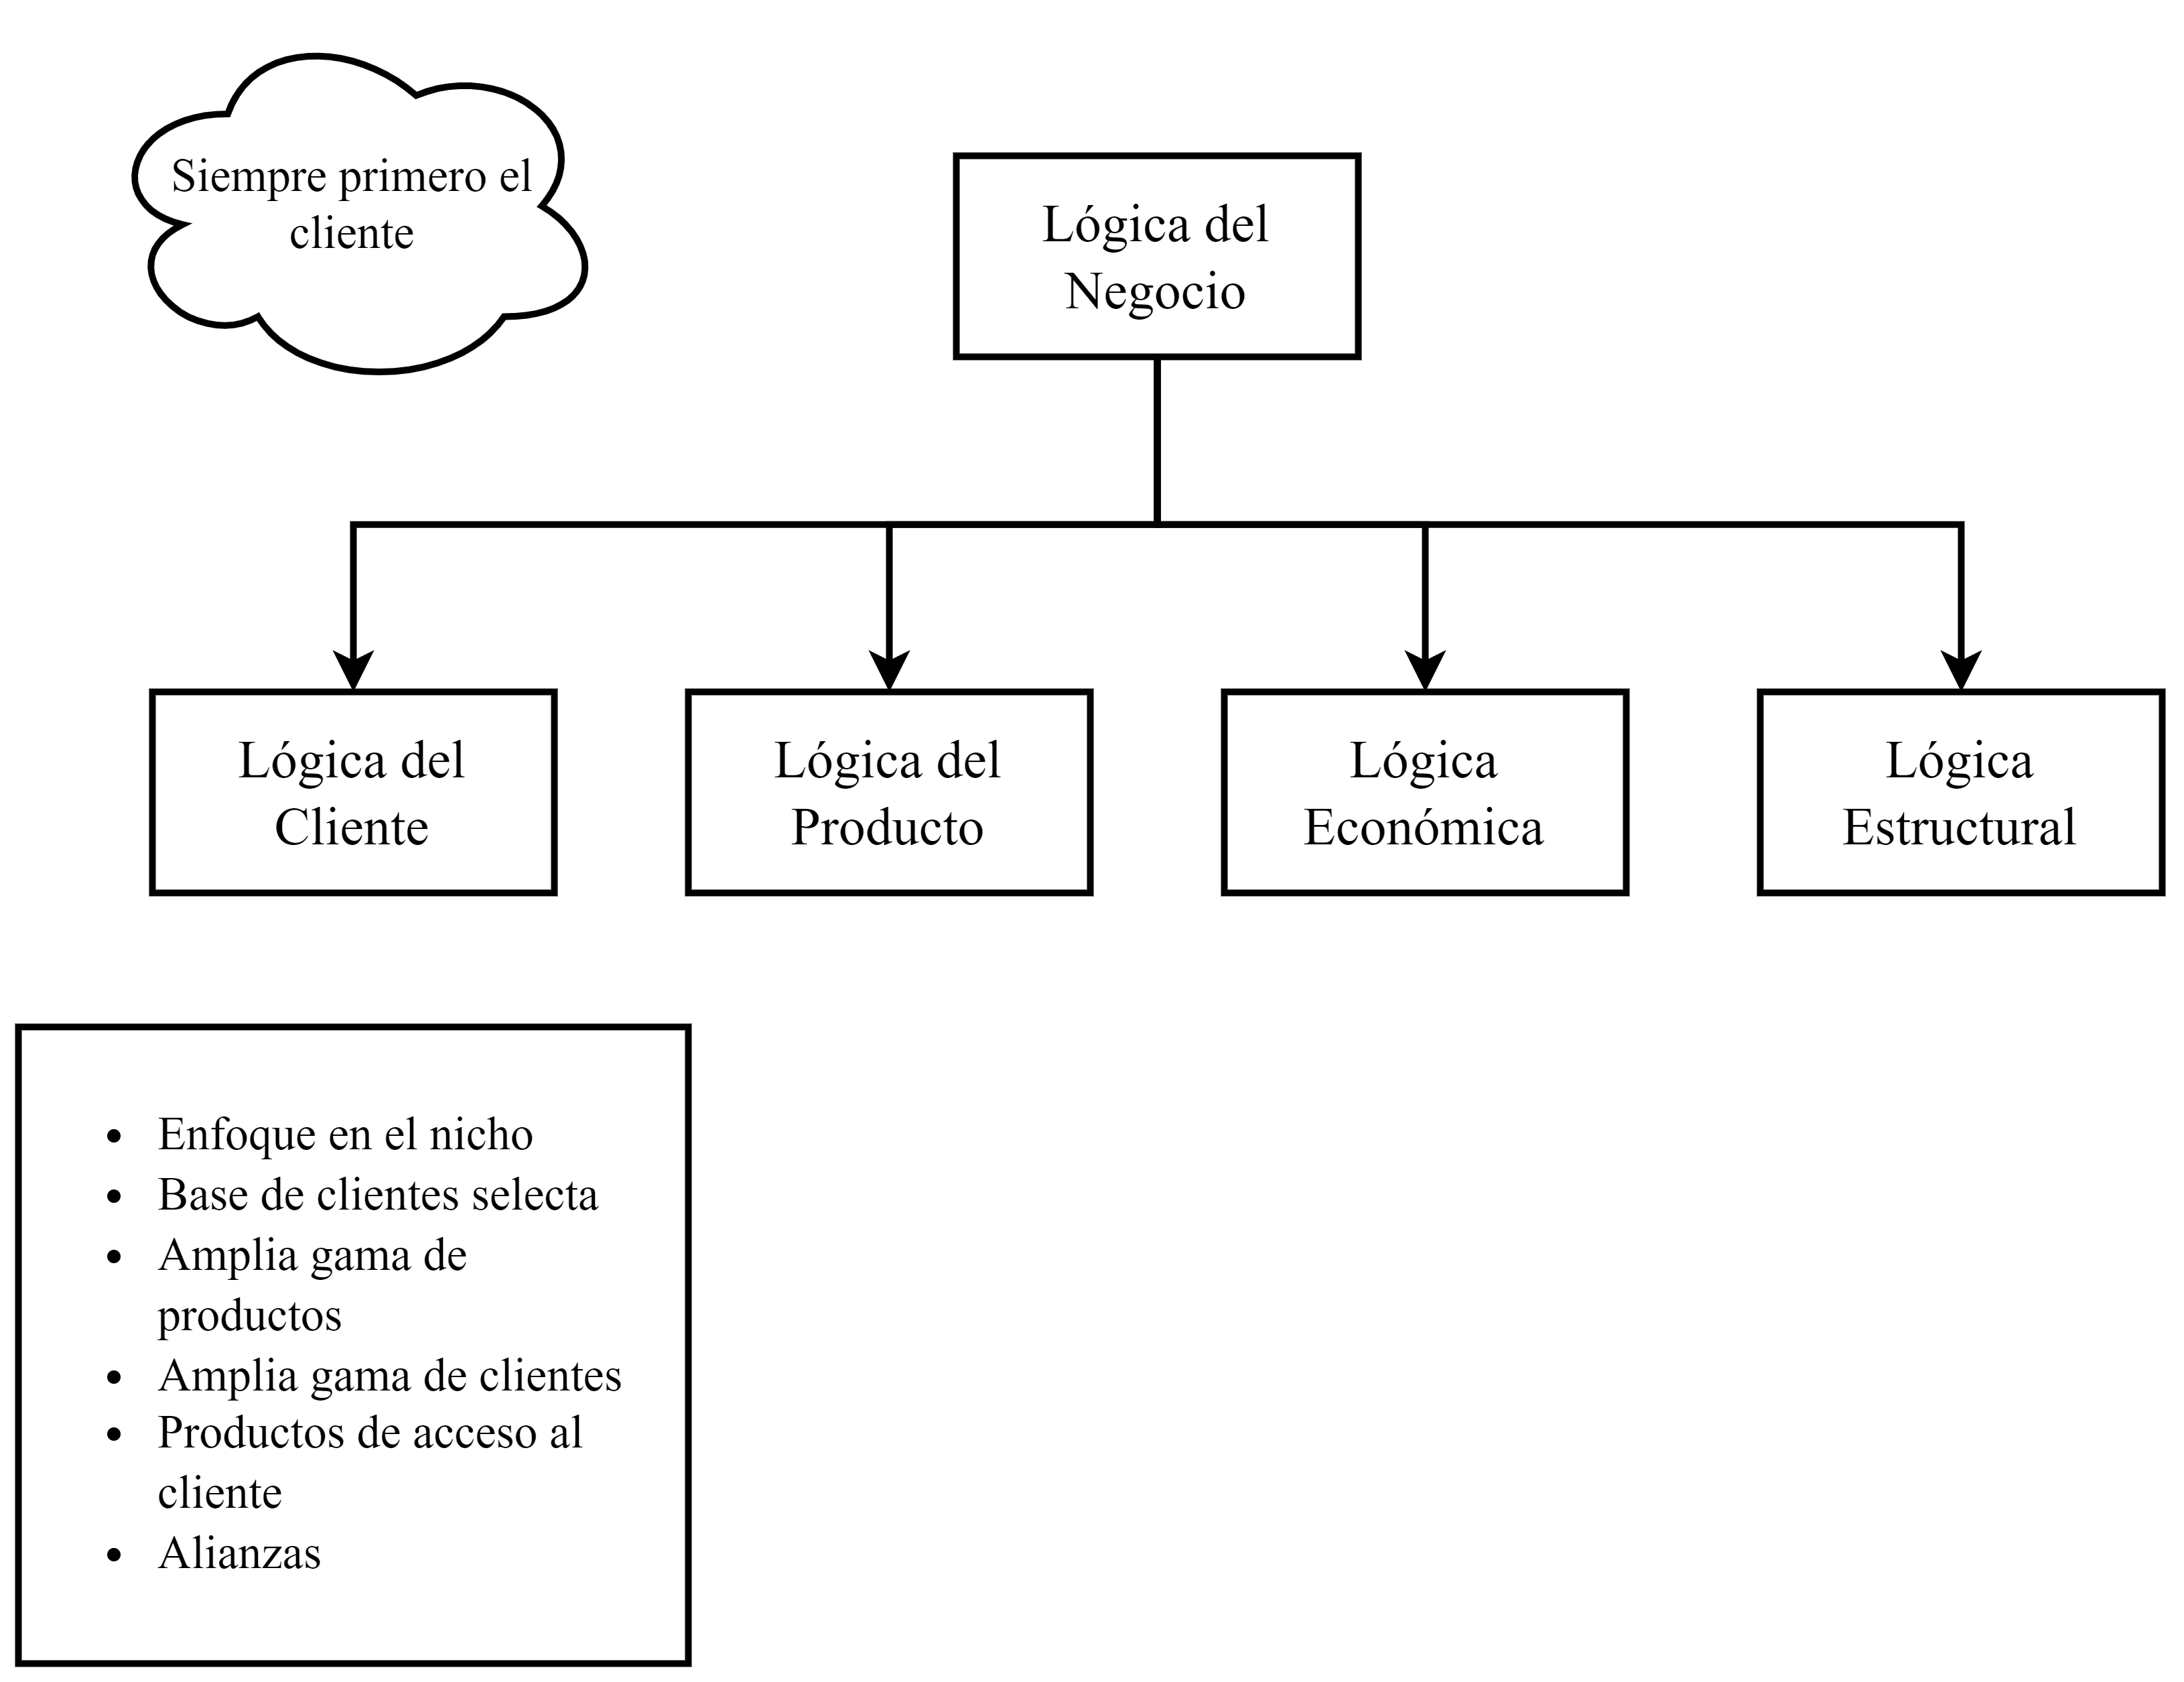
\includegraphics[width=\textwidth]{img/Logicas.png}
\end{figure}

\newpage
\subsubsection{Cadena de valor de negocios}
\begin{figure}[H]
    \centering
    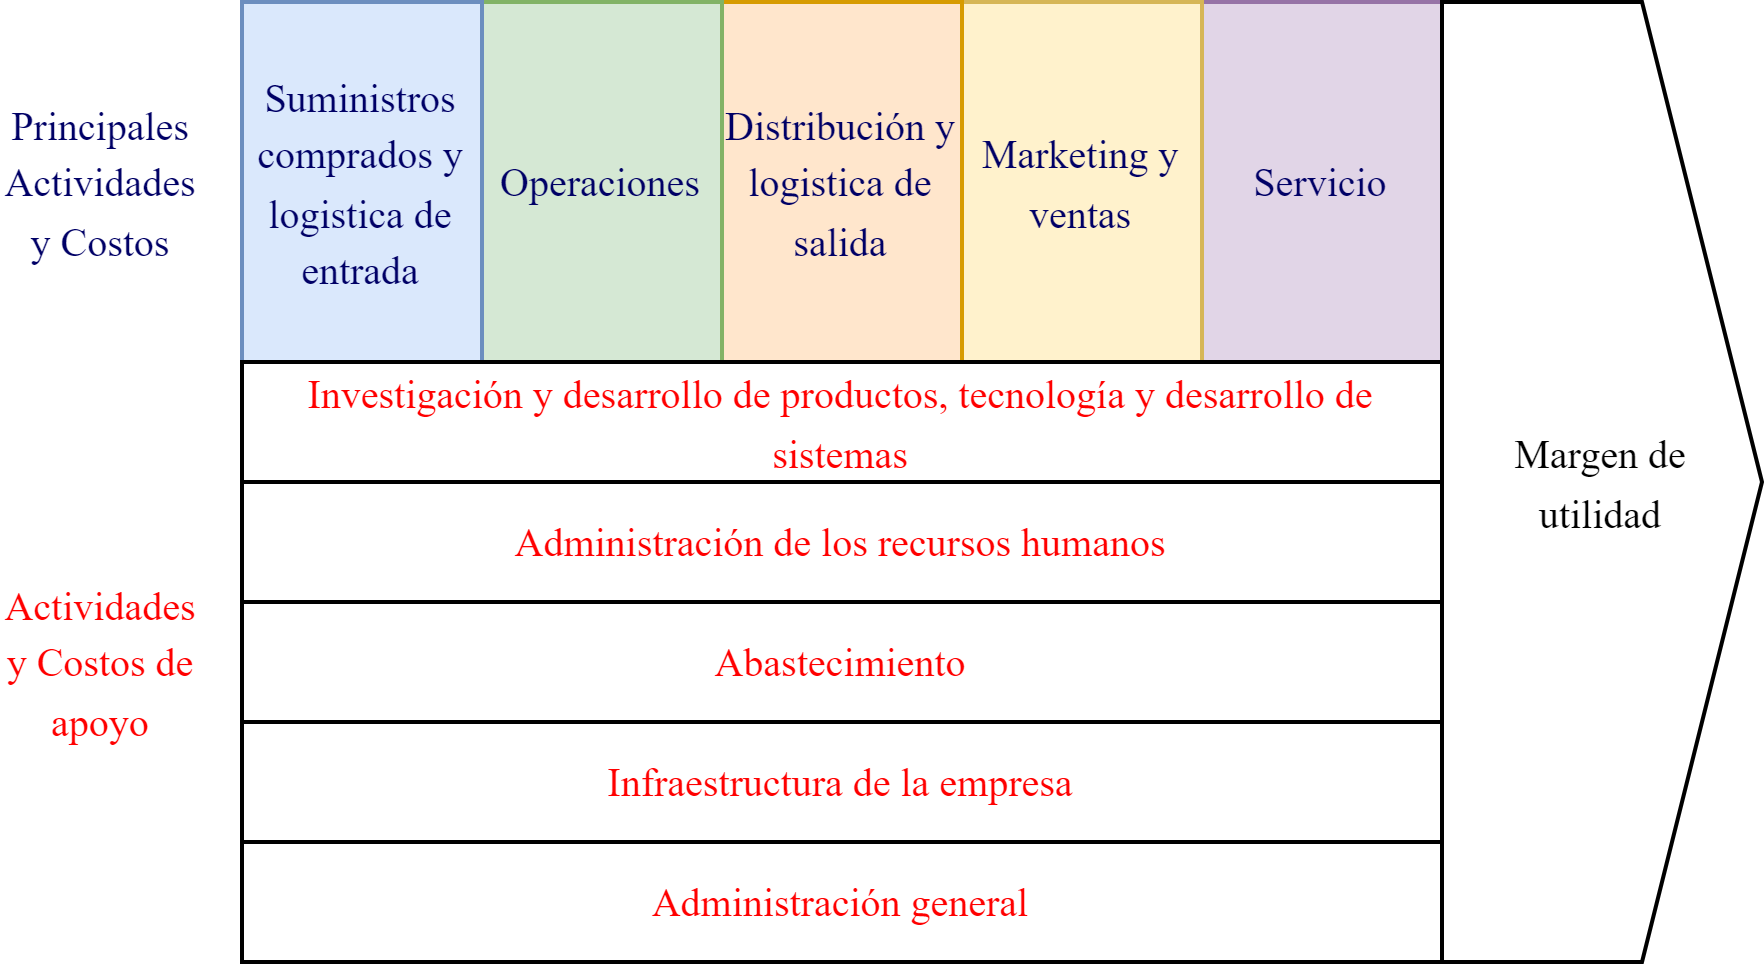
\includegraphics[width=1\textwidth]{img/costosdenoseque.png}
\end{figure}

\begin{itemize}
    \item El desglosar en este diagrama las operaciones de las actividades y procesos nos expone en gran medida los elementos que significan un costo para la empresa.
    \item Todas las actividades en la cadena de valor involucran un costo y limita activos.
    \item El asignar los costos de operación y activos a cada actividad nos permite ver un aproximado del costo respectivo.
    \item La cadena de valor y como se desempeñan las actividades reflejan la evolución del negocio, operaciones internas, estrategias, enfoques de ejecución y las economías de las actividades
\end{itemize}

\newpage
\section{Elección estratégica}\label{sec:eleccionEstrategica}
\subsection{Modelo de negocios}
Enfoque m\'as estrecho que la estrategia de negocios, esta vinculada con las iniciativa competitivas de la empresa y con los enfoques de negocios.
\newparagraph
El modelo de negocios tiene que ver con que los ingresos y costos asociados a la estrategia demuestran viabilidad de los negocios.
\newparagraph
\subitem - Las empresas con mas tiempo en los negocios con generación de utilidades tienen un modelo de negocios probado. Existe evidencia que su estrategia ha sido benéfica y que la empresa es viable
\newparagraph
\subitem - Las empresas con perdida de dinero o en iniciación de actividades siguen un modelo de negocio errado o aun no probado. No se ha demostrado que sus estrategias produzcan buenos resultados y sean viables.

\subsection{Proceso de formulación de estrategias}
\begin{enumerate}
    \item Identificar el proceso o elemento al que se le confeccionara una estrategia.
    
    \item Análisis FODA del proceso o elemento elegido.
    
    \item Identificar factores relevantes del proceso escogido.
    
    \item Decidir si utilizar:
    \begin{enumerate}
        \item 1 variable representativa.
        
        \item 2 o mas variables representativas.
    \end{enumerate}
    
    \item Definir resultados esperados de cada estrategia.
    
    \item Seleccionar estrategia/s mas viable/s.
    
    \item Elegir estrategia según objetivos planteados.
\end{enumerate}

\subsection{Estrategias}
\hypertarget{estrategia_corporativa}{\noindent\textbf{Nivel 1: \textit{Estrategias corporativas}}} \\
\indent Misión, vision, definición del negocio.
\begin{itemize}
    \item Liderazgo en costos.
    
    \item Diferenciación.
    
    \item Concentración.
\end{itemize}
\textbf{Nivel 2: \textit{Estrategias de cartera (productos - mercado)}} \newline
\textbf{Nivel 3: \textit{Estrategias de segmentación y posicionamiento}} \newline
\textbf{Nivel 4: \textit{Estrategias de funcionales}}

\subsubsection{Estrategias competitivas}
\noindent Dependiendo de la cuota de mercado que posea la empresa:
\begin{itemize}
    \item Estrategias de líder.
    
    \item Estrategias de retador.
    
    \item Estrategias de seguidor.
    
    \item Estrategias de especialista.
\end{itemize}

\subsubsection{Características de las empresas rentables}
\begin{itemize}
    \item Segmentar creativamente.
    
    \item Utilizar eficazmente variables investigación y desarrollo para disminuir costos y aumentar rentabilidad.
    
    \item Pensar en pequeño, conforme con su tamaño, poner acento en rentabilidad aprovechando su ventaja competitiva defendible.
    
    \item Fuerza del directivo que lo lleva a estar implicado, no sólo en la estrategia, sino también en la táctica.
\end{itemize}

\subsubsection{Estrategia corporativa}
\noindent Como se menciona en el \hyperlink{estrategia_corporativa}{Nivel 1}, la estrategia corporativa es la que establece el proposito y alcance de la empresa.
Su definición incluye dos decisiones trascendentes:
\begin{itemize}
    \item \textbf{Misión de la empresa}.
    
    \item \textbf{Definición del negocio.}
\end{itemize}
- Define las actividades en las que busca participar y su combinación mas adecuada.
- Busca sinergia entre la integración y complementariedad de las actividades de la cartera de negocio.

\newpage
\section{Certamen 1 - 2022} 
\subsection*{ITEM I (3 Ptos. c/u)}
Responda las siguientes aseveraciones, marcando con un “V” si la pregunta es verdadera o con una “F” si es 
falsa. Justifique las falsas.

\begin{enumerate}
    \item (\textcolor{green}{V}) El concepto de Estrategia implica un conjunto de decisiones y acciones que se llevan a cabo para lograr un determinado objetivo.
    
    \item (\textcolor{red}{F}) La Estrategia proyectada en una empresa es lo mismo que la Estrategia realizada.\newline
    \textcolor{blue}{
        La estrategia proyectada es el ideal, mientras que la estrategia realizada son las acciones que se llevan a cabo.
    }
    
    \item (\textcolor{green}{V}) Las características de la Administración Estratégica implican un proceso dinámico y participativo, compromiso de los jefes y transversal, entre otras.
    
    \item (\textcolor{green}{V}) El proceso de Administración Estratégica incluye la selección de la misión y objetivos principales, análisis del ambiente competitivo externo y del ambiente operativo interno.\newline
    \textcolor{blue}{
        Además de la formulación, implantación y control de estrategias.
    }
    \item (\textcolor{green}{V}) El triángulo de la estratégica contiene: el análisis estratégico, la elección y la implementación de la estrategia.
    
    \item (\textcolor{green}{V}) Las consecuencias de rivalidad entre los competidores existentes son disminución de precios, aumento de costos y reducción de rentabilidad.
    
    \item (\textcolor{green}{V}/\textcolor{red}{F}?) Los factores críticos de éxito son elementos que ayudan a la empresa a lograr los objetivos. 
    \textcolor{yellow}{
        NO lo pasamos.
    }
    \item (\textcolor{green}{V}) Los requisitos para el desarrollo de una estrategia son: Conocimientos, Capacidad para integración, Imaginación y lógica para elegir entre alternativas, entre otros.
    
    \item (\textcolor{red}{F}) Al hacer la exploración ambiental y los 8 ambientes críticos de una empresa forestal se pueden concluir los mismos análisis que para la UBB.\newline
    \textcolor{blue}{
        A pesar de que comparten los mismos ambientes críticos, las conclusiones optenidas de estos seran diferentes.
    }
    
    \item (\textcolor{red}{F}) Una Unidad Estratégica de Negocios pertenece a una empresa productiva y tiene sus propios competidores.\newline
    \textcolor{blue}{
        De forma directa no tiene competidores, pero si al pertener a una empresa.
    }
\end{enumerate}

\newpage
\subsection*{ITEM II (5 Ptos. c/u)}
Explique con un ejemplo, cada uno de los siguientes conceptos: 

\begin{enumerate}
    \item Unidad Estratégica de Negocios\newline
    \textcolor{red}{
        NO ME SUENA
    }
    
    \item Matriz de crecimiento-participación\newline
    \textcolor{blue}{
        En la Universidad del Bío-Bío.
        \begin{itemize}
            \item Estrella: Ingeniería Civil Informática.
            \item Interrogante: Medicina.
            \item Vaca lechera: Ingeniería Civil Industrial.
            \item Perro: Ingeniería en Maderas.
        \end{itemize}
    }
    
    \item Ciclo de vida del producto\newline
    \textcolor{blue}{
        En la etapa de:
        \begin{itemize}
            \item Introducción tenemos a Temu.
            \item Aceptación tenemos a Edenred.
            \item Madurez tenemos a Discord.
            \item Saturación tenemos a Zoom.
            \item Obsolescencia tenemos a Skype.
        \end{itemize}
    }
    
    \item Ventaja competitiva\newline
    \textcolor{blue}{
        Ofrecer un servicio de delivery de comida a domicilio, con un tiempo de entrega menor a 30 minutos.
    }
    
    \item Fuerzas competitivas de Porter
    \textcolor{blue}{
        \begin{itemize}
            \item Poder de negociación de los compradores: Cliente elige comprar en carrito de verduras informal, en vez de supermercado.
            \item Rivalidad entre competidores: WhatsApp añade una nueva función de videollamada, para competir con Telegram.
            \item Amenaza de productos sustitutos: Miel y Stevia como sustitutos del azúcar.
            \item Poder de negociación de los proveedores: Panaderia que vende pan a supermercados.
            \item Amenaza de nuevos competidores: Llegada de Uber a un pueblo con monopolio de taxis.
        \end{itemize}
    }
\end{enumerate}

\newpage
\section{Certamen 1 - 2023} 

\subsection*{ITEM I (3 Ptos. c/u)}
Responda las siguientes aseveraciones, marcando con un “V” si la pregunta es verdadera o con una “F” si es falsa. Justifique las falsas.   
\begin{enumerate}
    \item (\textcolor{red}{F}) El producto Estrella, le indica a una empresa que el mercado lo acepta y por lo tanto, éste le reporta una alta participación de mercado.\newline
    \textcolor{blue}{
        Y además tiene un alto crecimiento en el mercado.
    }
    
    \item (\textcolor{red}{F}) Cuando un producto está en la etapa de introducción en el mercado, la empresa prácticamente no tiene que invertir en publicidad.\newline
    \textcolor{blue}{
        Falso, ya que es necesario invertir en publicidad para dar a conocer el producto.
    }
    
    \item (\textcolor{green}{V}/\textcolor{red}{F}) El análisis FODA le sirve a las empresas para determinar el punto máximo de ganancias.\newline
    \textcolor{blue}{
        Falso, dado que el FODA es un análisis a nivel interno y externo que nos permite maximizar los puntos positivos y minimizar los negativos que afectan a la empresa.
    }
    
    \item (\textcolor{green}{V}) Las áreas funcionales de una empresa, son Finanzas \& Contabilidad, RRHH \& Administración, Producción y Comercialización \& Marketing.
    
    \item (\textcolor{green}{V}) El proceso de la administración estratégica contiene: selección de misión y objetivos, formulación de estrategias e implementación de la estrategia.\newline
    \textcolor{blue}{
        Además le falta el control de la estrategia, el análisis del entorno externo e interno de la empresa.
    }
    
    \item (\textcolor{green}{V}) El Modelo 'de' resumen de los elementos de la Dirección Estratégica son: Análisis Estratégico, Elección Estratégica e Implantación de la Estrategia.
    
    \item (\textcolor{green}{V}) El modelo de negocio de una empresa involucra sólo al entorno interno.
    
    \item (\textcolor{green}{V}) Un proceso de formulación de estrategias para una empresa, implica considerar el corto plazo.
    
    \item (\textcolor{red}{F}) El Análisis PESTA le sirve a una empresa para determinar el punto máximo de ganancias.
    \textcolor{blue}{
        Falso, ya que el análisis PESTA es un análisis a nivel externo que nos permite conocer el entorno en el que se encuentra la empresa.
    }
    
    \item (\textcolor{red}{F}) Una estrategia competitiva implica que la empresa tiene las máximas ganancias económicas del mercado.\newline
    \textcolor{blue}{
        Falso, ya que una estrategia competitiva implica que la empresa tiene una ventaja competitiva sobre sus competidores.
    }
\end{enumerate}

\newpage
\subsection*{ITEM II (5 Ptos. c/u)}
Explique con un ejemplo, cada uno de los siguientes conceptos:
\begin{enumerate}
    \item Estrategia Competitiva
    \textcolor{blue}{
        \begin{itemize}
            \item Lider: Walmart, con sus precios bajos y gran variedad de productos a nivel mundial.
            \item Retador: Unimarc, con sus precios bajos y gran variedad de productos a nivel nacional.
            \item Seguidor: Ganga, con sus precios bajos y con no tanta variedad de productos a nivel regional.
            \item Especialista: Confiteria Turquesa, precio accesible y productos especializados en importación turca.
        \end{itemize}
    }
    
    \item Segmentación del mercado.
    
    \item Fuerzas competitivas de Porter.\newline
    \textcolor{blue}{
        Lo mismo que en el certamen anterior.
    }
    
    \item Entorno de una empresa
    \textcolor{red}{
        Jodimos.
    }
    
    \item Análisis Estratégico\newline
    \textcolor{blue}{
        Suponiendo que se quiere abrir una empresa de comida rápida en un sector de la ciudad, se debe analizar:
        \begin{itemize}
            \item El entorno: Otros locales de comida rápida, proveedores de insumos, clientes potenciales, zona de ubicación.
            \item Expectativas y propósitos: Vender lo suficiente para tener mas beneficios que costos.
            \item Recursos: Insumos para la comida, personal, local, utensilios.
            \item Competencias: Personal con las capacidades aptas y tenga atención al cliente.
            \item Capacidades: Ofrecer productos y atención de calidad.
        \end{itemize}
    }
\end{enumerate}
\end{document}